\hypertarget{system_8c}{
\section{system.c File Reference}
\label{system_8c}\index{system.c@{system.c}}
}
Short routines for controlling the whole system and modules. 

{\tt \#include $<$avr/eeprom.h$>$}\par
{\tt \#include \char`\"{}system.h\char`\"{}}\par
{\tt \#include \char`\"{}menu.h\char`\"{}}\par


Include dependency graph for system.c:\nopagebreak
\begin{figure}[H]
\begin{center}
\leavevmode
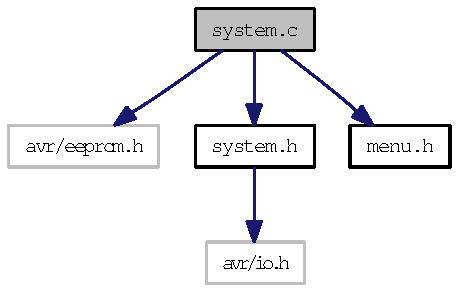
\includegraphics[width=128pt]{system_8c__incl}
\end{center}
\end{figure}
\subsection*{Functions}
\begin{CompactItemize}
\item 
void \hyperlink{system_8c_fcc5a33541d29a2d114643e67b7a5e68}{sys\_\-enter\_\-topmenu} ()
\begin{CompactList}\small\item\em Will set the current menu to the upper menu layer. \item\end{CompactList}\item 
void \hyperlink{system_8c_5e456b56f0c2ce2d53923272af0ad333}{sys\_\-enter\_\-submenu} ()
\begin{CompactList}\small\item\em Will set the current menu to to lower menu layer. \item\end{CompactList}\item 
void \hyperlink{system_8c_e2936ed52c758b103718c0101d5133df}{sys\_\-catcher\_\-disable} ()
\begin{CompactList}\small\item\em Diables (power off) the catcher stepper motor. \item\end{CompactList}\item 
void \hyperlink{system_8c_a740aed754b50165fb058dad9713f2f8}{sys\_\-catcher\_\-enable} ()
\begin{CompactList}\small\item\em Enables (power on) the catcher stepper motor. \item\end{CompactList}\item 
\hypertarget{system_8c_c8a68f0c5c371bc0f41e3ff4655eb9fa}{
void \hyperlink{system_8c_c8a68f0c5c371bc0f41e3ff4655eb9fa}{sys\_\-catcher\_\-move\_\-step} ()}
\label{system_8c_c8a68f0c5c371bc0f41e3ff4655eb9fa}

\begin{CompactList}\small\item\em Moves the catcher stepper motor for on step. \item\end{CompactList}\item 
void \hyperlink{system_8c_75278bd6ede508871b8d7880f24503d8}{sys\_\-catcher\_\-rotate} ()
\begin{CompactList}\small\item\em Rotates the catcher for one position. \item\end{CompactList}\item 
uint8\_\-t \hyperlink{system_8c_03ea663e9ae339039bc5cbcddee52d94}{sys\_\-get\_\-out\_\-pos} ()
\begin{CompactList}\small\item\em Gets the correct out index of the next to drop smartie. \item\end{CompactList}\item 
int8\_\-t \hyperlink{system_8c_60124c61aa7941fb311fdb4d85e6ba66}{sys\_\-catcher\_\-is\_\-lb\_\-blocked} ()
\begin{CompactList}\small\item\em Returns status for the catcher lightbarrier. \item\end{CompactList}\item 
void \hyperlink{system_8c_9fcb8a68acbcbb5ab57ca0ea752b5ad6}{sys\_\-revolver\_\-rotate} ()
\begin{CompactList}\small\item\em Rotates the revolver for one position. \item\end{CompactList}\item 
\hypertarget{system_8c_f98b8357b55993121effd5f8a144db21}{
void \hyperlink{system_8c_f98b8357b55993121effd5f8a144db21}{sys\_\-revolver\_\-move\_\-step} ()}
\label{system_8c_f98b8357b55993121effd5f8a144db21}

\begin{CompactList}\small\item\em Moves the revolver for one step. \item\end{CompactList}\item 
int8\_\-t \hyperlink{system_8c_768659fc9adb5f8edca3aed8711ef448}{sys\_\-revolver\_\-is\_\-lb\_\-blocked} ()
\begin{CompactList}\small\item\em Returns the status for the revolver lightbarrier. \item\end{CompactList}\item 
void \hyperlink{system_8c_851876925adec6a4c6d7cb6aec4bbbfd}{sys\_\-pause} ()
\begin{CompactList}\small\item\em Will Enter the pause mode. \item\end{CompactList}\item 
void \hyperlink{system_8c_6d65cab872ca8f9d37af4287ee012740}{sys\_\-reference\_\-measure\_\-blue} ()
\begin{CompactList}\small\item\em Initiates color callibration for corresponding smartie color. \item\end{CompactList}\item 
\hypertarget{system_8c_4ff06646314a1ccaf1947c9986c2486d}{
void \hyperlink{system_8c_4ff06646314a1ccaf1947c9986c2486d}{sys\_\-reference\_\-measure\_\-green} ()}
\label{system_8c_4ff06646314a1ccaf1947c9986c2486d}

\begin{CompactList}\small\item\em See \hyperlink{system_8h_6d65cab872ca8f9d37af4287ee012740}{sys\_\-reference\_\-measure\_\-blue} (). \item\end{CompactList}\item 
\hypertarget{system_8c_1ca664e0f0800b98f4e3cbb6295429ee}{
void \hyperlink{system_8c_1ca664e0f0800b98f4e3cbb6295429ee}{sys\_\-reference\_\-measure\_\-red} ()}
\label{system_8c_1ca664e0f0800b98f4e3cbb6295429ee}

\begin{CompactList}\small\item\em See \hyperlink{system_8h_6d65cab872ca8f9d37af4287ee012740}{sys\_\-reference\_\-measure\_\-blue} (). \item\end{CompactList}\item 
\hypertarget{system_8c_4dfe8d9daa9b136d3c7b5eb0c7d54489}{
void \hyperlink{system_8c_4dfe8d9daa9b136d3c7b5eb0c7d54489}{sys\_\-reference\_\-measure\_\-yellow} ()}
\label{system_8c_4dfe8d9daa9b136d3c7b5eb0c7d54489}

\begin{CompactList}\small\item\em See \hyperlink{system_8h_6d65cab872ca8f9d37af4287ee012740}{sys\_\-reference\_\-measure\_\-blue} (). \item\end{CompactList}\item 
\hypertarget{system_8c_430fcc5c084c5d195784456a4b0241fe}{
void \hyperlink{system_8c_430fcc5c084c5d195784456a4b0241fe}{sys\_\-reference\_\-measure\_\-orange} ()}
\label{system_8c_430fcc5c084c5d195784456a4b0241fe}

\begin{CompactList}\small\item\em See \hyperlink{system_8h_6d65cab872ca8f9d37af4287ee012740}{sys\_\-reference\_\-measure\_\-blue} (). \item\end{CompactList}\item 
\hypertarget{system_8c_5ede569de5e4adae83654eadf689319d}{
void \hyperlink{system_8c_5ede569de5e4adae83654eadf689319d}{sys\_\-reference\_\-measure\_\-brown} ()}
\label{system_8c_5ede569de5e4adae83654eadf689319d}

\begin{CompactList}\small\item\em See \hyperlink{system_8h_6d65cab872ca8f9d37af4287ee012740}{sys\_\-reference\_\-measure\_\-blue} (). \item\end{CompactList}\item 
\hypertarget{system_8c_ae77d91f8801da390b9dec1e4a740d85}{
void \hyperlink{system_8c_ae77d91f8801da390b9dec1e4a740d85}{sys\_\-reference\_\-measure\_\-purple} ()}
\label{system_8c_ae77d91f8801da390b9dec1e4a740d85}

\begin{CompactList}\small\item\em See \hyperlink{system_8h_6d65cab872ca8f9d37af4287ee012740}{sys\_\-reference\_\-measure\_\-blue} (). \item\end{CompactList}\item 
\hypertarget{system_8c_30d1084c81b5ad36c00bb9ee8fe9ac13}{
void \hyperlink{system_8c_30d1084c81b5ad36c00bb9ee8fe9ac13}{sys\_\-reference\_\-measure\_\-pink} ()}
\label{system_8c_30d1084c81b5ad36c00bb9ee8fe9ac13}

\begin{CompactList}\small\item\em See \hyperlink{system_8h_6d65cab872ca8f9d37af4287ee012740}{sys\_\-reference\_\-measure\_\-blue} (). \item\end{CompactList}\item 
void \hyperlink{system_8c_10b0d9845d6c021370b0d06a5a876205}{sys\_\-reference\_\-measure\_\-restore} ()
\begin{CompactList}\small\item\em Initiates to restore the color reference values. \item\end{CompactList}\item 
void \hyperlink{system_8c_73eeab714172d1723e3d412f36002a9b}{sys\_\-resume} ()
\begin{CompactList}\small\item\em Leave the pause mode. \item\end{CompactList}\item 
\hypertarget{system_8c_5ac3b5cf6f06e3ff4d3c745f9d5c693a}{
void \hyperlink{system_8c_5ac3b5cf6f06e3ff4d3c745f9d5c693a}{sys\_\-set\_\-speed} ()}
\label{system_8c_5ac3b5cf6f06e3ff4d3c745f9d5c693a}

\begin{CompactList}\small\item\em Set the operating speed of the sorter to the current demand value. \item\end{CompactList}\item 
void \hyperlink{system_8c_1826940cb85dc745f43b80c8554b3047}{sys\_\-speed\_\-up} ()
\begin{CompactList}\small\item\em Set the operating speed of the sorter up by decreasing pause times. \item\end{CompactList}\item 
void \hyperlink{system_8c_86167f37ad40f4c37766d17c9d07845d}{sys\_\-speed\_\-down} ()
\begin{CompactList}\small\item\em Set the operating speed of the sorter down by increasing pause times. \item\end{CompactList}\item 
\hypertarget{system_8c_4fdb3cc2b07ea1f4534bc1c3ac60a865}{
void \hyperlink{system_8c_4fdb3cc2b07ea1f4534bc1c3ac60a865}{sys\_\-measure\_\-tcs} ()}
\label{system_8c_4fdb3cc2b07ea1f4534bc1c3ac60a865}

\begin{CompactList}\small\item\em Initiate a color measurement with the tcs color sensor. \item\end{CompactList}\item 
\hypertarget{system_8c_0f47aa3043bc1362fbe37d003acfaf4e}{
void \hyperlink{system_8c_0f47aa3043bc1362fbe37d003acfaf4e}{sys\_\-measure\_\-adjd} ()}
\label{system_8c_0f47aa3043bc1362fbe37d003acfaf4e}

\begin{CompactList}\small\item\em Initiate a color measurement with the adjd color sensor. \item\end{CompactList}\item 
\hypertarget{system_8c_ef389e924ee5fb5cb82da6c6a11209b5}{
void \hyperlink{system_8c_ef389e924ee5fb5cb82da6c6a11209b5}{vibrator\_\-start} ()}
\label{system_8c_ef389e924ee5fb5cb82da6c6a11209b5}

\begin{CompactList}\small\item\em Initiates the vibrator to start. \item\end{CompactList}\item 
\hypertarget{system_8c_b2694695c165d073dd47850b83904682}{
void \hyperlink{system_8c_b2694695c165d073dd47850b83904682}{sensor\_\-adjd\_\-get\_\-color} ()}
\label{system_8c_b2694695c165d073dd47850b83904682}

\begin{CompactList}\small\item\em Initiates the color detection by the ADJD color sensor. \item\end{CompactList}\item 
\hypertarget{system_8c_895d4e598ce146273eb5dc50e5a140ea}{
void \hyperlink{system_8c_895d4e598ce146273eb5dc50e5a140ea}{sensor\_\-tcs\_\-get\_\-color} ()}
\label{system_8c_895d4e598ce146273eb5dc50e5a140ea}

\begin{CompactList}\small\item\em Initiates the color detection by the TCS color sensor. \item\end{CompactList}\item 
void \hyperlink{system_8c_97b11d5bfac2abcab58401879440e202}{catcher\_\-rotate\_\-absolute} (smartie\_\-color move\_\-to)
\begin{CompactList}\small\item\em Rotates the catcher to a certain position. \item\end{CompactList}\item 
void \hyperlink{system_8c_2c5ecc52ef42cf3086da340a8e3eae13}{catcher\_\-rotate\_\-relative} (int8\_\-t rel\_\-pos)
\begin{CompactList}\small\item\em Rotates the catcher from the current position to a relative next position regarding 'hole above hole'. \item\end{CompactList}\item 
void \hyperlink{system_8c_4312b8582a99de2443c53adce9359dc5}{revolver\_\-rotate\_\-relative} (int8\_\-t rel\_\-pos)
\begin{CompactList}\small\item\em Rotates the revolver from the current position to a relative next position regarding 'hole above hole'. \item\end{CompactList}\end{CompactItemize}


\subsection{Detailed Description}
Short routines for controlling the whole system and modules. 



Definition in file \hyperlink{system_8c-source}{system.c}.

\subsection{Function Documentation}
\hypertarget{system_8c_97b11d5bfac2abcab58401879440e202}{
\index{system.c@{system.c}!catcher\_\-rotate\_\-absolute@{catcher\_\-rotate\_\-absolute}}
\index{catcher\_\-rotate\_\-absolute@{catcher\_\-rotate\_\-absolute}!system.c@{system.c}}
\subsubsection{\setlength{\rightskip}{0pt plus 5cm}void catcher\_\-rotate\_\-absolute (smartie\_\-color {\em move\_\-to})}}
\label{system_8c_97b11d5bfac2abcab58401879440e202}


Rotates the catcher to a certain position. 

This function will rotate the catcher to position specified by the a color \hyperlink{system_8h_7b19b2744b17f8f369226dd73101a4b2}{smartie\_\-color\_\-t}. 

Definition at line 346 of file system.c.

References CATCH\_\-MAX\_\-SIZE, catcher\_\-rotate\_\-relative(), col\_\-unknown, stepper\_\-motor\_\-t::current\_\-pos, smartie\_\-sorter\_\-t::mot\_\-catcher, stat\_\-finished, and stepper\_\-motor\_\-t::status\_\-last.

Referenced by main().\hypertarget{system_8c_2c5ecc52ef42cf3086da340a8e3eae13}{
\index{system.c@{system.c}!catcher\_\-rotate\_\-relative@{catcher\_\-rotate\_\-relative}}
\index{catcher\_\-rotate\_\-relative@{catcher\_\-rotate\_\-relative}!system.c@{system.c}}
\subsubsection{\setlength{\rightskip}{0pt plus 5cm}void catcher\_\-rotate\_\-relative (int8\_\-t {\em rel\_\-pos})}}
\label{system_8c_2c5ecc52ef42cf3086da340a8e3eae13}


Rotates the catcher from the current position to a relative next position regarding 'hole above hole'. 

Most of the work is being done in \hyperlink{abstraction_8c_b45f6a6990e7755a39cc6279e3c09abf}{motor\_\-stuff}.

Warning: This function does not check if the catcher is already working. Before calling this function, check if the motor's status and last status equals \hyperlink{system_8h_6bfb87db0720ecda67ba06ab52162b035ad840e3bfeb7a8c1633431f009ec7fc}{stat\_\-idle}. It also doesn't check the parameter, if the value is reasonable.

\begin{Desc}
\item[Parameters:]
\begin{description}
\item[{\em rel\_\-pos}]The position where to move to. The value of rel\_\-pos will be not checked, so the value must be lower than \hyperlink{system_8h_388331d885423f07d4a701af481c62a7}{REV\_\-MAX\_\-SIZE} or \hyperlink{system_8h_ebeee5d587e924ad6d94000c311f24af}{CATCH\_\-MAX\_\-SIZE}. \end{description}
\end{Desc}


Definition at line 384 of file system.c.

References CATCH\_\-MAX\_\-SIZE, stepper\_\-motor\_\-t::current\_\-pos, smartie\_\-sorter\_\-t::mot\_\-catcher, stat\_\-finished, stat\_\-start\_\-working, stepper\_\-motor\_\-t::status, stepper\_\-motor\_\-t::status\_\-last, and stepper\_\-motor\_\-t::target\_\-pos.

Referenced by catcher\_\-rotate\_\-absolute(), init\_\-motors(), and sys\_\-catcher\_\-rotate().\hypertarget{system_8c_4312b8582a99de2443c53adce9359dc5}{
\index{system.c@{system.c}!revolver\_\-rotate\_\-relative@{revolver\_\-rotate\_\-relative}}
\index{revolver\_\-rotate\_\-relative@{revolver\_\-rotate\_\-relative}!system.c@{system.c}}
\subsubsection{\setlength{\rightskip}{0pt plus 5cm}void revolver\_\-rotate\_\-relative (int8\_\-t {\em rel\_\-pos})}}
\label{system_8c_4312b8582a99de2443c53adce9359dc5}


Rotates the revolver from the current position to a relative next position regarding 'hole above hole'. 

Most of the work is being done in \hyperlink{abstraction_8c_b45f6a6990e7755a39cc6279e3c09abf}{motor\_\-stuff}.

Warning: This function does not check if the revolver is already working. Before calling this function, check if the motor's status and last status equals \hyperlink{system_8h_6bfb87db0720ecda67ba06ab52162b035ad840e3bfeb7a8c1633431f009ec7fc}{stat\_\-idle}. It also doesn't check the parameter, if the value is reasonable.

\begin{Desc}
\item[Parameters:]
\begin{description}
\item[{\em rel\_\-pos}]The position where to move to. The value of rel\_\-pos will be not checked, so the value must be lower than \hyperlink{system_8h_388331d885423f07d4a701af481c62a7}{REV\_\-MAX\_\-SIZE} or \hyperlink{system_8h_ebeee5d587e924ad6d94000c311f24af}{CATCH\_\-MAX\_\-SIZE}. \end{description}
\end{Desc}


Definition at line 415 of file system.c.

References stepper\_\-motor\_\-t::current\_\-pos, smartie\_\-sorter\_\-t::mot\_\-revolver, REV\_\-MAX\_\-SIZE, stat\_\-finished, stat\_\-start\_\-working, stepper\_\-motor\_\-t::status, stepper\_\-motor\_\-t::status\_\-last, and stepper\_\-motor\_\-t::target\_\-pos.

Referenced by init\_\-motors(), main(), and sys\_\-revolver\_\-rotate().\hypertarget{system_8c_e2936ed52c758b103718c0101d5133df}{
\index{system.c@{system.c}!sys\_\-catcher\_\-disable@{sys\_\-catcher\_\-disable}}
\index{sys\_\-catcher\_\-disable@{sys\_\-catcher\_\-disable}!system.c@{system.c}}
\subsubsection{\setlength{\rightskip}{0pt plus 5cm}void sys\_\-catcher\_\-disable ()}}
\label{system_8c_e2936ed52c758b103718c0101d5133df}


Diables (power off) the catcher stepper motor. 

This function is prepared especially for functions started from the menu. This function works only if the menu is correct initialized. 

Definition at line 44 of file system.c.

References CATCH\_\-DISABLE.

Referenced by init\_\-motors().\hypertarget{system_8c_a740aed754b50165fb058dad9713f2f8}{
\index{system.c@{system.c}!sys\_\-catcher\_\-enable@{sys\_\-catcher\_\-enable}}
\index{sys\_\-catcher\_\-enable@{sys\_\-catcher\_\-enable}!system.c@{system.c}}
\subsubsection{\setlength{\rightskip}{0pt plus 5cm}void sys\_\-catcher\_\-enable ()}}
\label{system_8c_a740aed754b50165fb058dad9713f2f8}


Enables (power on) the catcher stepper motor. 

This function is prepared especially for functions started from the menu. This function works only if the menu is correct initialized. 

Definition at line 54 of file system.c.

References CATCH\_\-ENABLE.

Referenced by init\_\-motors().\hypertarget{system_8c_60124c61aa7941fb311fdb4d85e6ba66}{
\index{system.c@{system.c}!sys\_\-catcher\_\-is\_\-lb\_\-blocked@{sys\_\-catcher\_\-is\_\-lb\_\-blocked}}
\index{sys\_\-catcher\_\-is\_\-lb\_\-blocked@{sys\_\-catcher\_\-is\_\-lb\_\-blocked}!system.c@{system.c}}
\subsubsection{\setlength{\rightskip}{0pt plus 5cm}int8\_\-t sys\_\-catcher\_\-is\_\-lb\_\-blocked ()}}
\label{system_8c_60124c61aa7941fb311fdb4d85e6ba66}


Returns status for the catcher lightbarrier. 

This function is prepared especially for functions started from the menu. This function works only if the menu is correct initialized. 

Definition at line 98 of file system.c.

References IS\_\-LB\_\-CATCHER.

Referenced by init\_\-motors().\hypertarget{system_8c_75278bd6ede508871b8d7880f24503d8}{
\index{system.c@{system.c}!sys\_\-catcher\_\-rotate@{sys\_\-catcher\_\-rotate}}
\index{sys\_\-catcher\_\-rotate@{sys\_\-catcher\_\-rotate}!system.c@{system.c}}
\subsubsection{\setlength{\rightskip}{0pt plus 5cm}void sys\_\-catcher\_\-rotate ()}}
\label{system_8c_75278bd6ede508871b8d7880f24503d8}


Rotates the catcher for one position. 

This function is intened for manual usage and should not be used during normal running mode \hyperlink{system_8h_6e4cea4b6246f491c526211f5405627d564529220e61e848983d8eb9d7f87736}{SYS\_\-MODE\_\-RUNNING}, only during \hyperlink{system_8h_6e4cea4b6246f491c526211f5405627df1c8a041b6d3d46002d02ed0645a8ba2}{SYS\_\-MODE\_\-PAUSE}. 

Definition at line 72 of file system.c.

References catcher\_\-rotate\_\-relative(), smartie\_\-sorter\_\-t::mot\_\-catcher, smartie\_\-sorter\_\-t::prog, prog\_\-rotate\_\-catcher, stat\_\-idle, stepper\_\-motor\_\-t::status, and stepper\_\-motor\_\-t::status\_\-last.

Referenced by init\_\-menu().\hypertarget{system_8c_5e456b56f0c2ce2d53923272af0ad333}{
\index{system.c@{system.c}!sys\_\-enter\_\-submenu@{sys\_\-enter\_\-submenu}}
\index{sys\_\-enter\_\-submenu@{sys\_\-enter\_\-submenu}!system.c@{system.c}}
\subsubsection{\setlength{\rightskip}{0pt plus 5cm}void sys\_\-enter\_\-submenu ()}}
\label{system_8c_5e456b56f0c2ce2d53923272af0ad333}


Will set the current menu to to lower menu layer. 

This function is prepared especially for functions started from the menu. This function works only if the menu is correct initialized. 

Definition at line 33 of file system.c.

References smartie\_\-sorter\_\-t::prog, prog\_\-none, and menu\_\-entry\_\-t::submenu.

Referenced by init\_\-menu().\hypertarget{system_8c_fcc5a33541d29a2d114643e67b7a5e68}{
\index{system.c@{system.c}!sys\_\-enter\_\-topmenu@{sys\_\-enter\_\-topmenu}}
\index{sys\_\-enter\_\-topmenu@{sys\_\-enter\_\-topmenu}!system.c@{system.c}}
\subsubsection{\setlength{\rightskip}{0pt plus 5cm}void sys\_\-enter\_\-topmenu ()}}
\label{system_8c_fcc5a33541d29a2d114643e67b7a5e68}


Will set the current menu to the upper menu layer. 

This function is prepared especially for functions started from the menu. This function works only if the menu is correct initialized. 

Definition at line 22 of file system.c.

References smartie\_\-sorter\_\-t::prog, prog\_\-none, and menu\_\-entry\_\-t::topmenu.

Referenced by init\_\-menu().\hypertarget{system_8c_03ea663e9ae339039bc5cbcddee52d94}{
\index{system.c@{system.c}!sys\_\-get\_\-out\_\-pos@{sys\_\-get\_\-out\_\-pos}}
\index{sys\_\-get\_\-out\_\-pos@{sys\_\-get\_\-out\_\-pos}!system.c@{system.c}}
\subsubsection{\setlength{\rightskip}{0pt plus 5cm}uint8\_\-t sys\_\-get\_\-out\_\-pos ()}}
\label{system_8c_03ea663e9ae339039bc5cbcddee52d94}


Gets the correct out index of the next to drop smartie. 

\begin{Desc}
\item[Returns:]The index of smartie in the revolver which will be dropped next \end{Desc}


Definition at line 85 of file system.c.

References stepper\_\-motor\_\-t::current\_\-pos, smartie\_\-sorter\_\-t::mot\_\-revolver, and REV\_\-MAX\_\-SIZE.

Referenced by main().\hypertarget{system_8c_851876925adec6a4c6d7cb6aec4bbbfd}{
\index{system.c@{system.c}!sys\_\-pause@{sys\_\-pause}}
\index{sys\_\-pause@{sys\_\-pause}!system.c@{system.c}}
\subsubsection{\setlength{\rightskip}{0pt plus 5cm}void sys\_\-pause ()}}
\label{system_8c_851876925adec6a4c6d7cb6aec4bbbfd}


Will Enter the pause mode. 

This function will enter the pause mode after the current function is finished. This function is usually called from the lcd menu. This function is only available in the mode \hyperlink{system_8h_6e4cea4b6246f491c526211f5405627d564529220e61e848983d8eb9d7f87736}{SYS\_\-MODE\_\-RUNNING} 

Definition at line 149 of file system.c.

References system\_\-state\_\-t::mode, system\_\-state\_\-t::mode\_\-last, smartie\_\-sorter\_\-t::state, and SYS\_\-MODE\_\-PAUSE.

Referenced by init\_\-menu().\hypertarget{system_8c_6d65cab872ca8f9d37af4287ee012740}{
\index{system.c@{system.c}!sys\_\-reference\_\-measure\_\-blue@{sys\_\-reference\_\-measure\_\-blue}}
\index{sys\_\-reference\_\-measure\_\-blue@{sys\_\-reference\_\-measure\_\-blue}!system.c@{system.c}}
\subsubsection{\setlength{\rightskip}{0pt plus 5cm}void sys\_\-reference\_\-measure\_\-blue ()}}
\label{system_8c_6d65cab872ca8f9d37af4287ee012740}


Initiates color callibration for corresponding smartie color. 

This function is prepared especially for functions started from the menu. This function works only if the menu is correct initialized. 

Definition at line 163 of file system.c.

References smartie\_\-sorter\_\-t::prog, and prog\_\-set\_\-colors\_\-blue.

Referenced by init\_\-menu().\hypertarget{system_8c_10b0d9845d6c021370b0d06a5a876205}{
\index{system.c@{system.c}!sys\_\-reference\_\-measure\_\-restore@{sys\_\-reference\_\-measure\_\-restore}}
\index{sys\_\-reference\_\-measure\_\-restore@{sys\_\-reference\_\-measure\_\-restore}!system.c@{system.c}}
\subsubsection{\setlength{\rightskip}{0pt plus 5cm}void sys\_\-reference\_\-measure\_\-restore ()}}
\label{system_8c_10b0d9845d6c021370b0d06a5a876205}


Initiates to restore the color reference values. 

This function is prepared especially for functions started from the menu. This function works only if the menu is correct initialized. 

Definition at line 222 of file system.c.

References smartie\_\-sorter\_\-t::prog, and prog\_\-set\_\-colors\_\-restore.

Referenced by init\_\-menu().\hypertarget{system_8c_73eeab714172d1723e3d412f36002a9b}{
\index{system.c@{system.c}!sys\_\-resume@{sys\_\-resume}}
\index{sys\_\-resume@{sys\_\-resume}!system.c@{system.c}}
\subsubsection{\setlength{\rightskip}{0pt plus 5cm}void sys\_\-resume ()}}
\label{system_8c_73eeab714172d1723e3d412f36002a9b}


Leave the pause mode. 

This function will leave the pause mode. This function is usually called from the lcd menu. This function is only available in the mode \hyperlink{system_8h_6e4cea4b6246f491c526211f5405627df1c8a041b6d3d46002d02ed0645a8ba2}{SYS\_\-MODE\_\-PAUSE} 

Definition at line 233 of file system.c.

References system\_\-state\_\-t::mode, system\_\-state\_\-t::mode\_\-last, smartie\_\-sorter\_\-t::state, and SYS\_\-MODE\_\-RUNNING.

Referenced by init\_\-menu().\hypertarget{system_8c_768659fc9adb5f8edca3aed8711ef448}{
\index{system.c@{system.c}!sys\_\-revolver\_\-is\_\-lb\_\-blocked@{sys\_\-revolver\_\-is\_\-lb\_\-blocked}}
\index{sys\_\-revolver\_\-is\_\-lb\_\-blocked@{sys\_\-revolver\_\-is\_\-lb\_\-blocked}!system.c@{system.c}}
\subsubsection{\setlength{\rightskip}{0pt plus 5cm}int8\_\-t sys\_\-revolver\_\-is\_\-lb\_\-blocked ()}}
\label{system_8c_768659fc9adb5f8edca3aed8711ef448}


Returns the status for the revolver lightbarrier. 

This function is prepared especially for functions started from the menu. This function works only if the menu is correct initialized. 

Definition at line 138 of file system.c.

References IS\_\-LB\_\-REVOLVER.

Referenced by init\_\-motors().\hypertarget{system_8c_9fcb8a68acbcbb5ab57ca0ea752b5ad6}{
\index{system.c@{system.c}!sys\_\-revolver\_\-rotate@{sys\_\-revolver\_\-rotate}}
\index{sys\_\-revolver\_\-rotate@{sys\_\-revolver\_\-rotate}!system.c@{system.c}}
\subsubsection{\setlength{\rightskip}{0pt plus 5cm}void sys\_\-revolver\_\-rotate ()}}
\label{system_8c_9fcb8a68acbcbb5ab57ca0ea752b5ad6}


Rotates the revolver for one position. 

This function is intened for manual usage and should not be used during normal running mode \hyperlink{system_8h_6e4cea4b6246f491c526211f5405627d564529220e61e848983d8eb9d7f87736}{SYS\_\-MODE\_\-RUNNING}, only during \hyperlink{system_8h_6e4cea4b6246f491c526211f5405627df1c8a041b6d3d46002d02ed0645a8ba2}{SYS\_\-MODE\_\-PAUSE}. 

Definition at line 118 of file system.c.

References smartie\_\-sorter\_\-t::mot\_\-revolver, smartie\_\-sorter\_\-t::prog, prog\_\-rotate\_\-revolver, revolver\_\-rotate\_\-relative(), stat\_\-idle, stepper\_\-motor\_\-t::status, and stepper\_\-motor\_\-t::status\_\-last.

Referenced by init\_\-menu().\hypertarget{system_8c_86167f37ad40f4c37766d17c9d07845d}{
\index{system.c@{system.c}!sys\_\-speed\_\-down@{sys\_\-speed\_\-down}}
\index{sys\_\-speed\_\-down@{sys\_\-speed\_\-down}!system.c@{system.c}}
\subsubsection{\setlength{\rightskip}{0pt plus 5cm}void sys\_\-speed\_\-down ()}}
\label{system_8c_86167f37ad40f4c37766d17c9d07845d}


Set the operating speed of the sorter down by increasing pause times. 

This function is prepared especially for functions started from the menu. This function works only if the menu is correct initialized. 

Definition at line 269 of file system.c.

References smartie\_\-sorter\_\-t::prog, smartie\_\-sorter\_\-t::speed, and sys\_\-set\_\-speed().

Referenced by init\_\-menu().\hypertarget{system_8c_1826940cb85dc745f43b80c8554b3047}{
\index{system.c@{system.c}!sys\_\-speed\_\-up@{sys\_\-speed\_\-up}}
\index{sys\_\-speed\_\-up@{sys\_\-speed\_\-up}!system.c@{system.c}}
\subsubsection{\setlength{\rightskip}{0pt plus 5cm}void sys\_\-speed\_\-up ()}}
\label{system_8c_1826940cb85dc745f43b80c8554b3047}


Set the operating speed of the sorter up by decreasing pause times. 

This function is prepared especially for functions started from the menu. This function works only if the menu is correct initialized. 

Definition at line 256 of file system.c.

References smartie\_\-sorter\_\-t::prog, smartie\_\-sorter\_\-t::speed, and sys\_\-set\_\-speed().

Referenced by init\_\-menu().